\section{Ramsey Numbers}

Everything so far has asked when a coloring exists. The opposite question is at least as natural: how large does a structure have to be before every coloring of it is forced to contain something monochromatic? Let's step back into ``graph land'' from ``hypergraph land'' and ask it of the complete graphs, coloring edges this time rather than vertices.

\begin{boxdefinition}[Ramsey Number]
    The $k$th Ramsey number, denoted $R(k)$, is the smallest $n \in \N$ such that any $2$-coloring of edges of $K_n$ gives a monochromatic $K_k$.
\end{boxdefinition}

One immediate result we can see is that $R(3) \geq 6$, which we can see simply by drawing a picture of $K_5$ and studying what happens if we move our attention to $K_6$.

\begin{figure}[H]
    \centering
    \begin{tikzpicture}[scale = 2]
        \begin{scope}[red]
            \stepedges{5}{1}
        \end{scope}
        \begin{scope}[blue]
            \stepedges{5}{2}
        \end{scope}
        \cyclevertices{5}
    \end{tikzpicture}
\end{figure}

Each color carries a $5$-cycle---the outer pentagon in red, the inner pentagram in blue---and a $5$-cycle contains no triangle at all, so neither color gives us a monochromatic $K_3$. Nothing forces a monochromatic triangle at $n = 5$, and so $R(3) \geq 6$. The picture also shows how little room there is to spare: every vertex of $K_5$ meets exactly two edges of each color, and the moment we pass to $K_6$ each vertex has five edges to distribute between two colors, so one of the colors is forced to take three of them.

We can actually prove that $R(3) = 6$, but this is rather nontrivial.

Other known Ramsey numbers are $R(2) = 2$ and $R(4) = 18$. The rest are unknown, though we do have bounds for them. The best (or close to the best) known bounds are
\begin{align*}
    2^{\frac{k}{2}} \leq R(k) \leq 3.8^k
\end{align*}

Upper bounds of this kind come from a recursion, which is cleanest stated for the off-diagonal Ramsey number $R(k, \ell)$: the smallest $n \in \N$ such that any red/blue coloring of the edges of $K_n$ gives a red $K_k$ or a blue $K_\ell$, so that $R(k) = R(k, k)$.

\begin{boxtheorem} \label{Ch2:Thm:Ramsey_Recursion}
    For all $k, \ell \geq 2$, we have
    \begin{align*}
        R(k, \ell) \leq R(k - 1, \ell) + R(k, \ell - 1)
    \end{align*}
\end{boxtheorem}

See undergraduate graph theory notes. \todo{add cross-ref to Michele's notes}

\subsection{Hypergraph Ramsey Numbers}

Nothing in the question needs the things being colored to be the edges of a graph, and our motivation for going further is the following result about sequences, which we state without proof.

\begin{boxtheorem}[\Erdos-Szekeres]
    If $n \geq \parenth{r - 1}\parenth{s - 1} + 1$, then any real sequence $a_1, \ldots, a_n$ has a non-decreasing subsequence of length $r$ or a decreasing subsequence of length $s$.
\end{boxtheorem}

To ask the question of hypergraphs we need the hypergraph with every possible hyper-edge.

\begin{boxdefinition}[Complete Uniform Hypergraph]
    Define the \textbf{complete $r$-uniform hypergraph on $n$ vertices}, denoted $K_{(r)}(n)$, to be the $r$-hypergraph on $n$ vertices with all possible hyper-edges.
\end{boxdefinition}

What we look for inside it is the analogue of a monochromatic $K_k$.

% [CORRECTED] was: "a colouring on that hypergraph", and "any red/blue colouring of $K_{(r)}(n)$" in the next box ---
% a coloring of a hypergraph colors its vertices in these notes (the definition in 2.1.2, Colorings of
% Hypergraphs), and read that way $R_{(r)}(k, \ell)$ would be $k + \ell - 1$ whenever $k, \ell \geq r$, whatever
% $r$ is; the proof below colors hyper-edges, and $R_{(2)}(k, k)$ is $R(k)$ only if they are.
% [CORRECTED] was: "The \textbf{size} of a $k$-clique is the number of edges." --- every use of size counts vertices:
% the arguments of $R_{(r)}$ do, and the clique of size $A = R_{(r)}(k - 1, \ell)$ in the proof below is what $R_{(r - 1)}$
% produces, which is $A$ vertices and $\binom{A}{r - 1}$ hyper-edges.
\begin{boxdefinition}[$k$-clique]
    Given a hypergraph and a coloring of its hyper-edges, a \textbf{$k$-clique of some color} is a set  of $k$ vertices such that all possible hyper-edges on that vertex set are monochromatic, of that color. The \textbf{size} of a $k$-clique is its number of vertices, $k$.
\end{boxdefinition}

The Ramsey numbers of graphs then generalize directly.

\begin{boxdefinition}[Hypergraph Ramsey Number]
    Given $r, k, \ell \in \N$, we define $R_{(r)}(k, \ell)$ to be the least $n$ such that any red/blue coloring of the hyper-edges of $K_{(r)}(n)$ contains a red $k$-clique or a blue $\ell$-clique.
\end{boxdefinition}

For small $r$ these are familiar objects. $K_{(2)}(n)$ is just $K_n$, so $R_{(2)}(k, k)$ is the Ramsey number $R(k)$ above, and in $K_{(1)}(n)$ each vertex is a hyper-edge by itself. Below are $K_{(1)}(4)$, $K_{(2)}(4)$ and $K_{(3)}(4)$, the last with its four hyper-edges drawn as triangles: three shaded ones, and the outline of the fourth around them.

\begin{figure}[H]
    \centering
    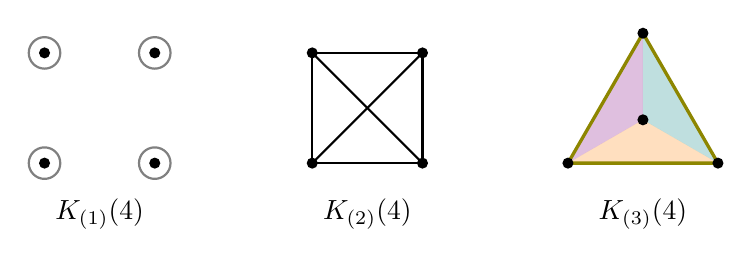
\begin{tikzpicture}
        \foreach \x/\y in {0/0, 1.4/0, 1.4/1.4, 0/1.4}{
            \draw[thick, gray] (\x, \y) circle (0.2);
            \fill[black] (\x, \y) circle (2pt);
        }
        \node at (0.7, -0.65) {$K_{(1)}(4)$};
        \begin{scope}[xshift = 3.4cm]
            \draw[thick] (0, 0) -- (1.4, 0) -- (1.4, 1.4) -- (0, 1.4) -- cycle;
            \draw[thick] (0, 0) -- (1.4, 1.4);
            \draw[thick] (1.4, 0) -- (0, 1.4);
            \foreach \x/\y in {0/0, 1.4/0, 1.4/1.4, 0/1.4}{
                \fill[black] (\x, \y) circle (2pt);
            }
            \node at (0.7, -0.65) {$K_{(2)}(4)$};
        \end{scope}
        \begin{scope}[xshift = 7.6cm, yshift = 0.55cm]
            \fill[violet, opacity = 0.25] (90:1.1) -- (210:1.1) -- (0, 0) -- cycle;
            \fill[orange, opacity = 0.25] (210:1.1) -- (330:1.1) -- (0, 0) -- cycle;
            \fill[teal, opacity = 0.25] (330:1.1) -- (90:1.1) -- (0, 0) -- cycle;
            \draw[olive, very thick] (90:1.1) -- (210:1.1) -- (330:1.1) -- cycle;
            \foreach \a in {90, 210, 330}{
                \fill[black] (\a:1.1) circle (2pt);
            }
            \fill[black] (0, 0) circle (2pt);
            \node at (0, -1.2) {$K_{(3)}(4)$};
        \end{scope}
    \end{tikzpicture}
\end{figure}

Once the hyper-edges are colored, a clique of a color is a set of vertices all of whose hyper-edges have that color: in the coloring of $K_{(2)}(4)$ below, the red triangle is a red $3$-clique, and each blue edge is a blue $2$-clique.

\begin{figure}[H]
    \centering
    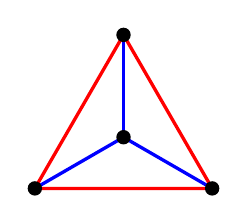
\begin{tikzpicture}[scale = 1.3]
        \draw[very thick, red] (90:1) -- (210:1) -- (330:1) -- cycle;
        \foreach \a in {90, 210, 330}{
            \draw[very thick, blue] (0, 0) -- (\a:1);
            \fill[black] (\a:1) circle (2pt);
        }
        \fill[black] (0, 0) circle (2pt);
    \end{tikzpicture}
\end{figure}

One easy fact to see is the following.

\begin{boxlemma} \label{Ch2:Lemma:Hypergraph_Ramsey_1}
    $R_{(1)}(k, \ell) = k + \ell - 1$.
\end{boxlemma}
\begin{proof}
    % [FILLED] proof supplied here; the lecture stated the lemma without proving it
    In $K_{(1)}(n)$ every hyper-edge is a single vertex, so coloring the hyper-edges colors the vertices, and a red $k$-clique is just $k$ red vertices. If $n \geq k + \ell - 1$, then fewer than $k$ red vertices leaves at least $\ell$ blue ones. If $n \leq k + \ell - 2$, coloring at most $k - 1$ vertices red and at most $\ell - 1$ blue gives neither.
\end{proof}

\subsection{A Recursive Upper Bound}

We can compute a similar bound to what we know about Ramsey numbers on graphs (\Cref{Ch2:Thm:Ramsey_Recursion}).

% [CORRECTED] was: "For all $r, k, \ell$" --- the right-hand side needs $R_{(r - 1)}$, $R_{(r)}(k - 1, \cdot)$ and $R_{(r)}(\cdot, \ell - 1)$,
% and these definitions give the first only for $r \geq 2$ and the others only for $k, \ell \geq 2$.
\begin{boxtheorem} \label{Ch2:Thm:Hypergraph_Ramsey_Recursion}
    For all $r, k, \ell \geq 2$, we have
    \begin{align*}
        R_{(r)}(k, \ell) \le R_{(r - 1)}\of{R_{(r)}\of{k - 1, \ell}, R_{(r)}\of{k, \ell - 1}} + 1
    \end{align*}
\end{boxtheorem}
\begin{proof}
    Write $A = R_{(r)}(k - 1, \ell)$ and $B = R_{(r)}(k, \ell - 1)$, and take $n = R_{(r - 1)}(A, B) + 1$.

    % [CORRECTED] was: "It has $R_{(n - 1)}\of{A, B}$ neighbours." (the $n - 1$ a slip for $r - 1$), and $H$ with no vertex set named --- when $n < r$, as at
    % $r = 3$ and $k = \ell = 2$, $K_{(r)}(n)$ has no hyper-edges and $v$ no neighbors; what the proof uses is the $n - 1$ other vertices.
    Consider $K_{(r)}(n)$, the complete $r$-uniform hypergraph on $[n]$. Consider any red/blue coloring of its edges. Fix $v \in V\of{K_{(r)}(n)}$. There are $R_{(r - 1)}\of{A, B}$ other vertices.

    % [CORRECTED] was: "removing $v$ from every edge" --- the edges missing $v$ would survive with $r$ vertices, so $H$ would
    % not be $(r - 1)$-uniform, and $R_{(r - 1)}$ could not be applied to it.
    Denote by $H$ the $(r - 1)$-uniform hypergraph on those vertices made by removing $v$ from every edge containing $v$. Every $(r - 1)$-subset $S$ of those vertices is the shadow $\parenth{S \cup \set{v}} \setminus \set{v}$ of exactly one edge, so $H$ is a copy of $K_{(r - 1)}(n - 1)$. Define a ``shadow coloring'' of $H$ by letting the color of the ``shadow edge'' $f \setminus \set{v}$ be just the color of $f$.

    By induction/definition of $R_{(r - 1)}$, the shadow contains either a red clique of size $A$ or a blue clique of size $B$.

    \begin{description}
        \item[\underline{Case A: Shadow coloring has a red clique of size $A$.}] Let $W$ be its vertex set, so that $\abs{W} = A = R_{(r)}(k - 1, \ell)$ and every $r$-set $S \cup \set{v}$ with $S$ an $(r - 1)$-subset of $W$ is red. The original coloring of the $r$-subsets of $W$ is a red/blue coloring of a copy of $K_{(r)}(A)$, so $W$ contains either a blue $\ell$-clique, and we are done, or a red $(k - 1)$-clique $U$. In the second case $U \cup \set{v}$ is a red $k$-clique: an $r$-subset of it either lies inside $U$, and is red because $U$ is a red clique, or is $S \cup \set{v}$ for an $(r - 1)$-subset $S$ of $U \ssq W$, and is red because $W$ is a red clique of the shadow.
        \item[\underline{Case B: Shadow coloring has a blue clique of size $B$.}] The same argument with the colors exchanged: its vertex set has $B = R_{(r)}(k, \ell - 1)$ vertices, so it contains either a red $k$-clique, and we are done, or a blue $(\ell - 1)$-clique $U$, and then $U \cup \set{v}$ is a blue $\ell$-clique.
    \end{description}

    Either way, the coloring has a red $k$-clique or a blue $\ell$-clique, so $R_{(r)}(k, \ell) \leq n = R_{(r - 1)}(A, B) + 1$.
\end{proof}

% [FILLED] this paragraph, the corollary and its proof supplied on the author's request (2026-09-30), not from the lecture
At $r = 2$ the bound, together with \Cref{Ch2:Lemma:Hypergraph_Ramsey_1}, reads $R(k, \ell) \leq R(k - 1, \ell) + R(k, \ell - 1)$, which is \Cref{Ch2:Thm:Ramsey_Recursion}. More importantly, the recursion is what shows that these numbers exist at all: the definition asks for a least $n$, and nothing so far has produced even one.

\begin{boxcorollary} \label{Ch2:Cor:Hypergraph_Ramsey_Finite}
    For all $r, k, \ell \in \N$, the Ramsey number $R_{(r)}(k, \ell)$ exists.
\end{boxcorollary}
\begin{proof}
    Induct on $r$. The case $r = 1$ is \Cref{Ch2:Lemma:Hypergraph_Ramsey_1}. For $r \geq 2$, induct on $k + \ell$. If $k = 1$ or $\ell = 1$, then $R_{(r)}(k, \ell) = 1$, since a single vertex has no $r$-subsets and so is vacuously a clique of both colors. Otherwise $k, \ell \geq 2$, so $R_{(r)}(k - 1, \ell)$ and $R_{(r)}(k, \ell - 1)$ exist by the induction on $k + \ell$, $R_{(r - 1)}$ of them exists by the induction on $r$, and the proof of \Cref{Ch2:Thm:Hypergraph_Ramsey_Recursion} exhibits an $n$ with the required property.
\end{proof}
